\documentclass{report}
\usepackage[margin=1in, paperwidth=8.5in, paperheight=11in]{geometry}
%Math packages%
\usepackage{amsmath}
\usepackage{amsthm}
%Spacing%
\usepackage{setspace}
%Package to adjust indentation%
\usepackage{changepage}
\onehalfspacing
%Lecture number%
\newcommand{\lectureNum}{23}
%Variables - Date and Course%
\newcommand{\curDate}{March 30, 2017}
\newcommand{\course}{CS 240}
%Defining the example tag%
%\theoremstyle{definition}%
\newtheorem{ex}{Example}[section]
%Setting counter given the lecture number%
\setcounter{chapter}{\lectureNum{}}
%Package to insert code%
\usepackage{listings}
\usepackage{courier}
\usepackage{xcolor}
\lstset { 
    tabsize=2,
    breaklines=true,
    language=C++,
    backgroundcolor=\color{blue!8}, % set backgroundcolor
    basicstyle=\footnotesize\ttfamily,% basic font setting
}
%Package to draw trees%
\usepackage{tikz}


\begin{document}
%Note title%
\begin{center}
\begin{Large}
\textsc{\course{} | Lecture \lectureNum{}}
\end{Large}
\end{center} 
\noindent \textit{Bartosz Antczak} \hfill
\textit{Instructor: Eric Schost} \hfill
\textit{\curDate{}}
\rule{\textwidth}{0.4pt}
% Actual Notes%
\section{More on B-trees}
\subsection{Height of a B-tree}
The height of a tree with $n$ nodes is $\Theta((\log n)/(\log M))$.
For the exam, know the algorithms that can be applied on this tree (delete, search, insert), and also know that the height of a tree is $\Theta((\log n)/(\log M))$.
\subsubsection{Proof of the height of a B-tree}
$M$ is the maximum number of children for any node. With that in mind, observe that the number of keys $n$ in the tree is
\begin{align*}
n &\geq {\left(\frac{M}{2}\right)}^h \\
\log(n) &\geq h \log \left(\frac{M}{2}\right) \\
\frac{\log(n)}{\log(\frac{M}{2})} &\geq h\\
h &\in O\left(\frac{\log(n)}{\log(M)}\right)
\end{align*}
Similarly we have:
\begin{align*}
n &\leq M^{h+1} \\
\log(n) &\leq (h+1) \log(M) \\
h &\in \Omega\left(\frac{\log(n)}{\log(M)}\right)
\end{align*}
Thus, we have $h \in \Theta\left(\frac{\log(n)}{\log(M)}\right)$
\subsection{Hashing in External Memory}
How can we hash and minimize disk transfers? We can use \textbf{extendible hashing}, which is similar to a B-tree with height 1 and max size $S$ at the leaves.
\subsubsection{Structure}
The directory is stored in internal memory. It contains an array of size $2^d$, where $d$ is called the \textit{order}.\\
Each directory entry points to a block stored in external memory. Each block contains at most $S$ items. Note that many entries can point to the same block. The values in every block in block $B$ agree on leading $k_B$ bits:
\begin{figure}[ht]
\begin{center}
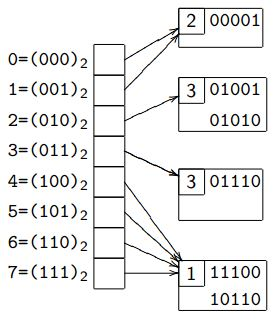
\includegraphics[scale=0.7]{hash.jpg}
\end{center}
\end{figure}
Know how the data structure is constructed. How to search. How to insert items. FORGET ABOUT DELETE.
%END%
\end{document}